\quad Poniżej przedstawiona jest tabela średniego czasu klasyfikacji na 
zbiorze testowym specjalnie dla tego celu (zbiór ma ogromną ilość punktów).
$10^6$ losowych punktów $(x, y)$ w przestrzeni $\mathbb{R}^2$, gdzie $(x, y) \in \left[-10^{14},10^{14}\right]^{2}$.
\begin{lstlisting}
    test_set = generate_uniform_points(-10^4, 10^4, 10 ** 6)
\end{lstlisting}
\begin{figure}[htb]
    \centering 
    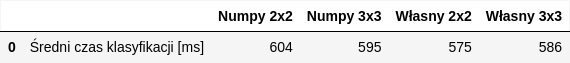
\includegraphics[scale=0.6]{wyz.png}\par
    \caption*{Tabela 5: Czasy klasyfikacji na zbiorze testowym. }
\end{figure}
\quad Widzimy ogromne różnice w czasach klasyfikacji naszego zbioru dla różnych wyznaczników. 
Najbardziej oczywistą różnicą jest różnica pomiędzy wyznacznikami napisanymi ręcznie, a 
funkcjami bibliotecznymi, z których ostatnie demonstrują dużo gorsze czasy. 
Prawdopodobnie możemy zaobserwować takie zjawisko dlatego, że funkcje biblioteczne implementują dużo większy zakres 
narzędzi, przez co pod czas wielokrotnego wywołania tej samej funkcji są wolniejsze w porównaniu do 
kilku prostych operacji arytmetycznych, którymi są nasze funkcje liczące wyznacznik. 